\newpage
%\section{Results}
\chapter{Results}
\label{sec:results}
\section{Synthesis}
\label{sec:synthesis_results}
All synthesis results in this chapter are synthesized for $Pixel\_Data\_Width$ of 16, unless another value is 
especially mentioned. Results presented in this chapter are gathered from synthesis utilization reports.
\subsection{Shiftregister}
\textbf{Shiftregister} was synthesized for $P\_bands$=10,20,30,40,50,60,70,80,90,100. Number of synthesized Slice registers and Slice LUTs are shown in Figure \ref{fig:primitives_shiftregister}. 

\begin{figure}[H]

\hbox{\hspace*{-2cm}                                                           
   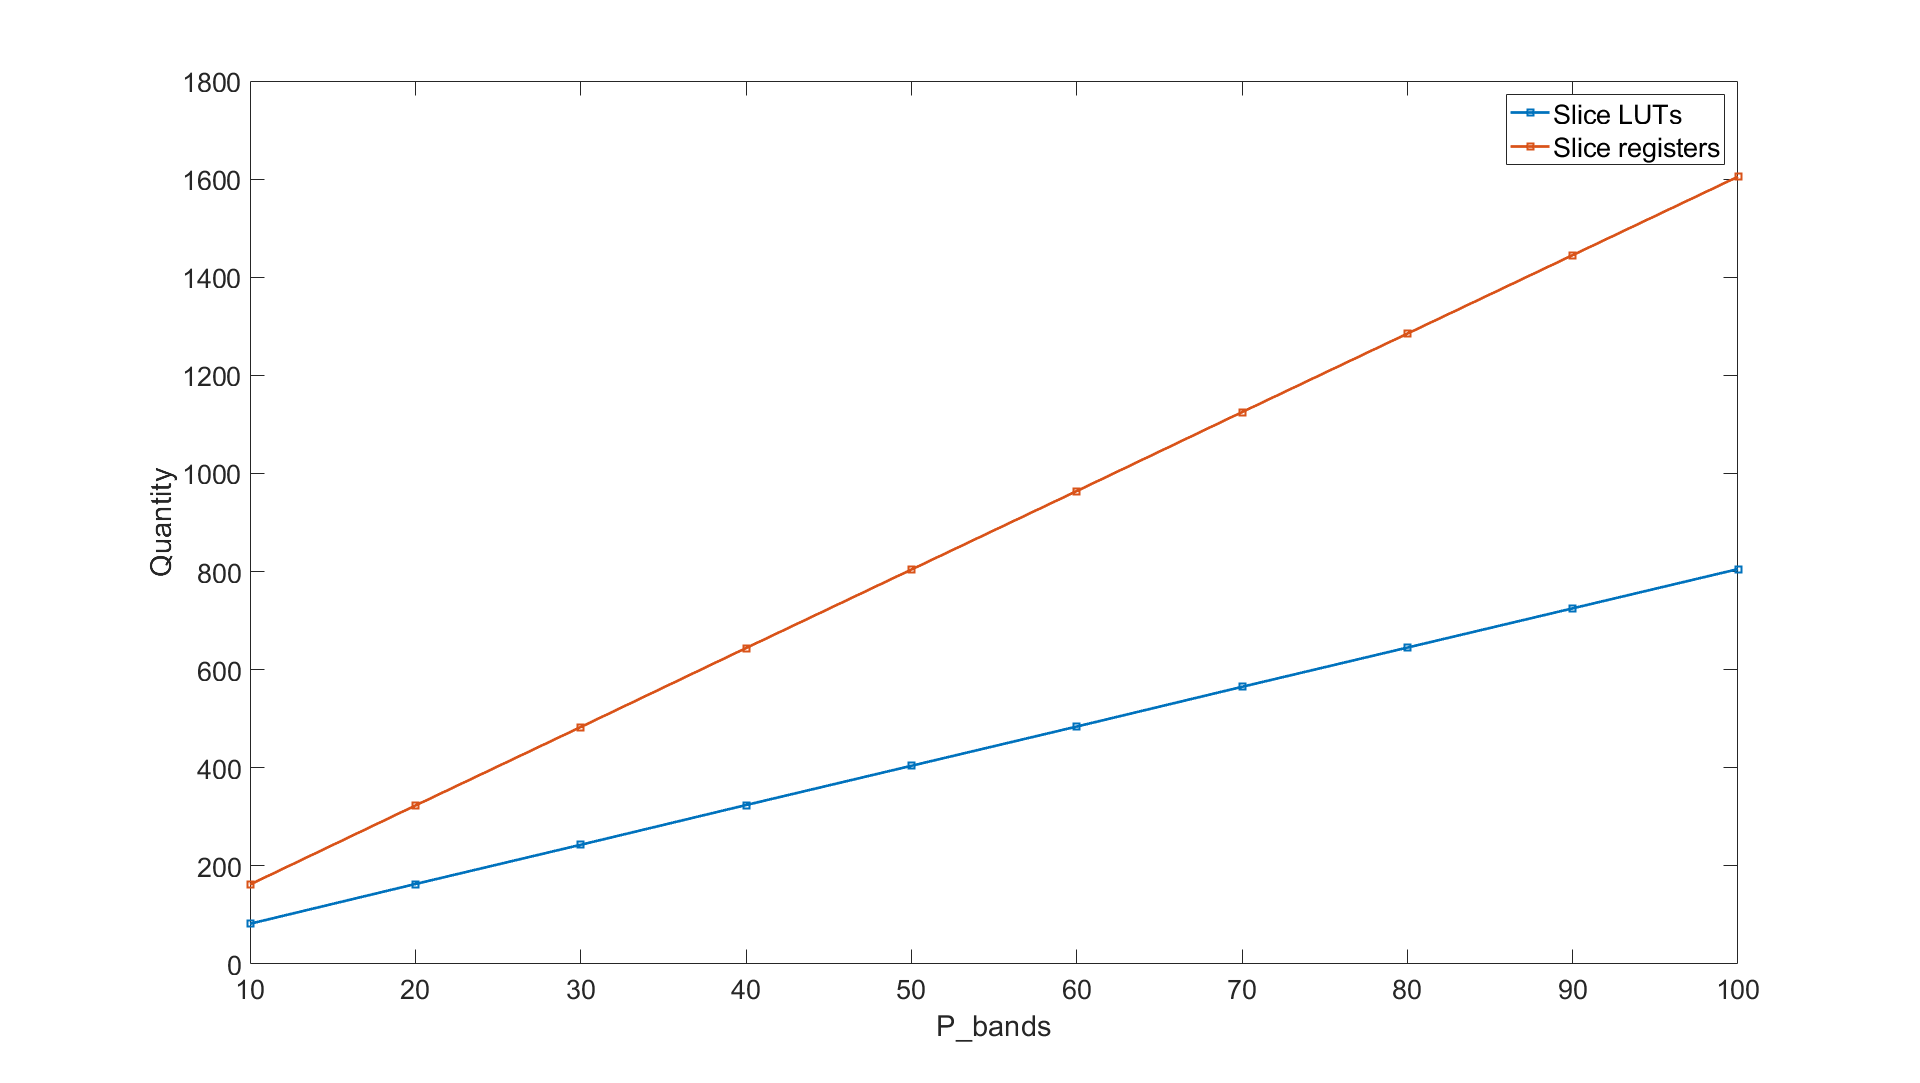
\includegraphics[scale=0.3]{images/syntese_resultat/shiftregister.png}}
  \caption{\textbf{Shiftregister} synthesis results.  } 
  \label{fig:primitives_shiftregister}
\end{figure}

\subsection{ACAD correlation}

The design was synthesized for $P\_bands$= [10, 20, 30, 40, 50, 60, 70, 80, 90, 100]. Figure \ref{fig:primitves_correlation}  shows the number of synthesized BRAM36E1 and DSP48E1. Figure \ref{fig:luts_and_regs_corr} shows number of synthesized Slice Registers and Slice LUTs as a function of $P\_bands$.

\begin{figure}[H]

\hbox{\hspace*{-2cm}                                                           
   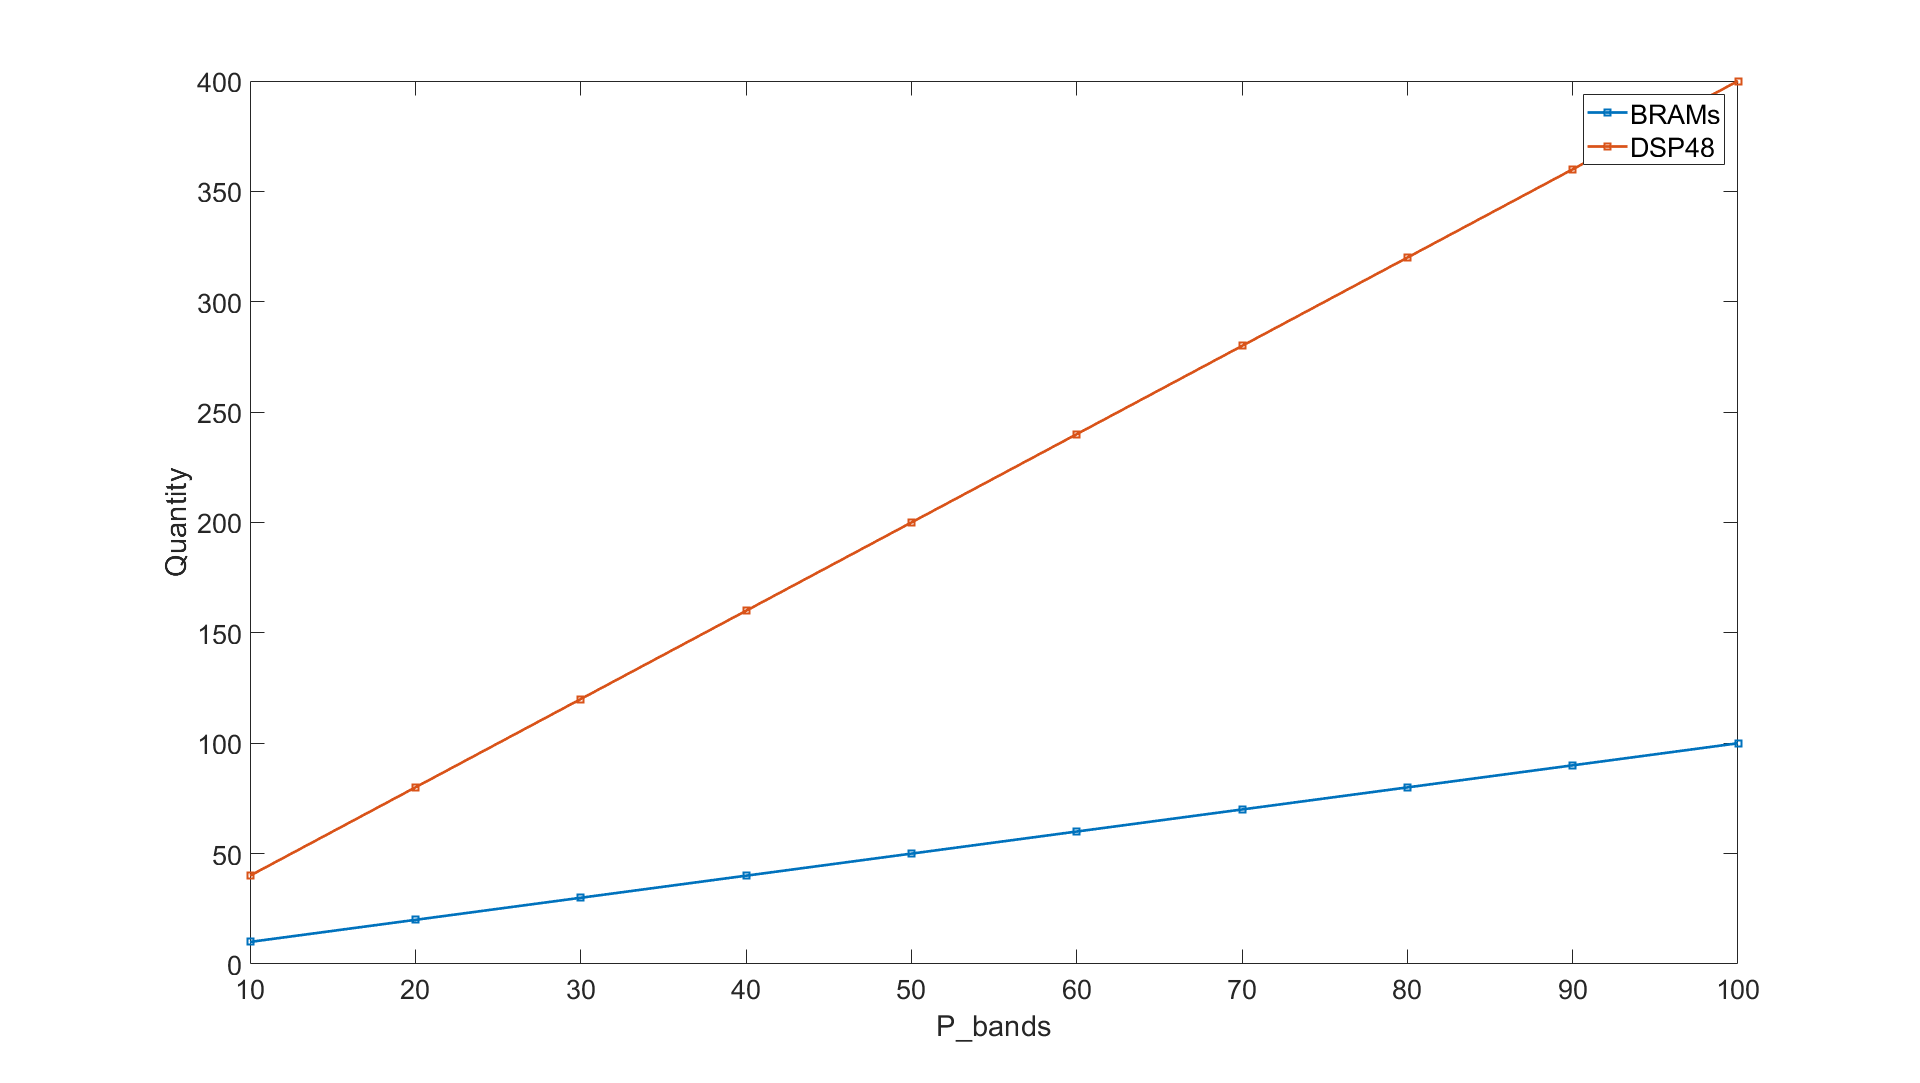
\includegraphics[scale=0.3]{images/number_of_BRAMS_and_DSP48_correlation_module.png}}
  \caption{Number of synthesized BRAM36E1 and DSP48E1 as a function of $P\_bands$ for the \textbf{ACAD correlation} block.  } 
  \label{fig:primitves_correlation}
\end{figure}


\begin{figure}[H]

\hbox{\hspace*{-2cm}                                                           
   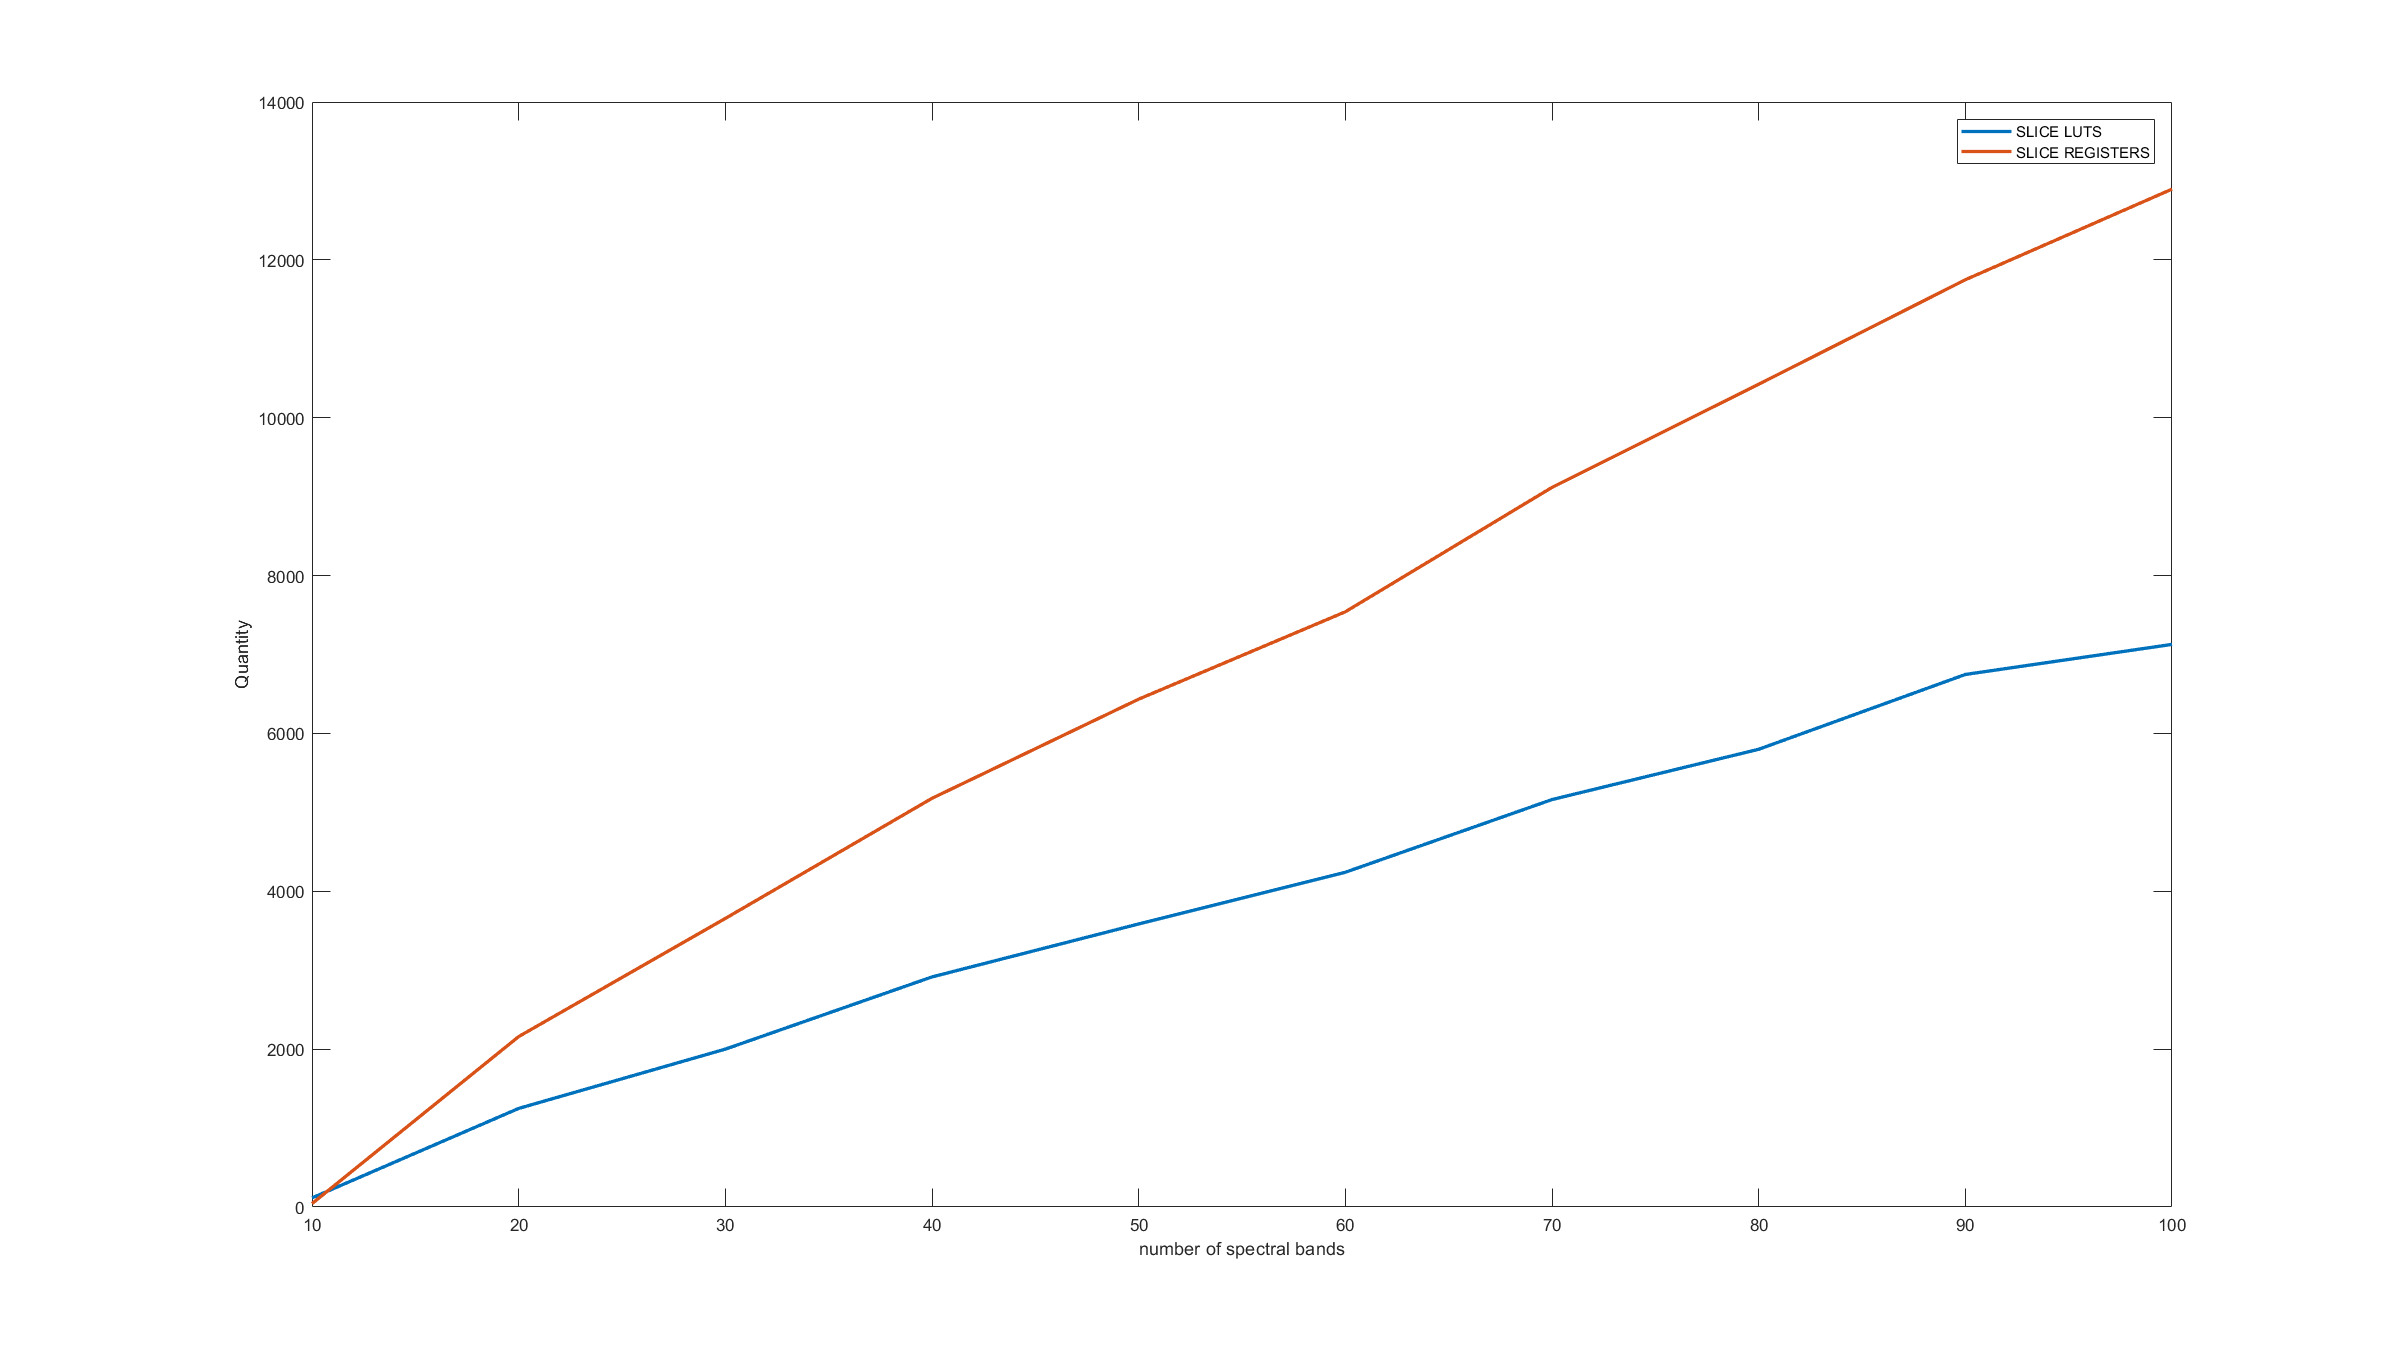
\includegraphics[scale=0.3]{images/correlation_luts_and_registers.png}}
  \caption{Number of synthesized SLICE REGISTERS and Slice LUTs as a function of $P\_bands$ for the \textbf{ACAD correlation} block. } 
  \label{fig:luts_and_regs_corr}
\end{figure}

 

\subsection{Inverse}



\begin{figure}[H]

\hbox{\hspace*{-1cm}                                                           
   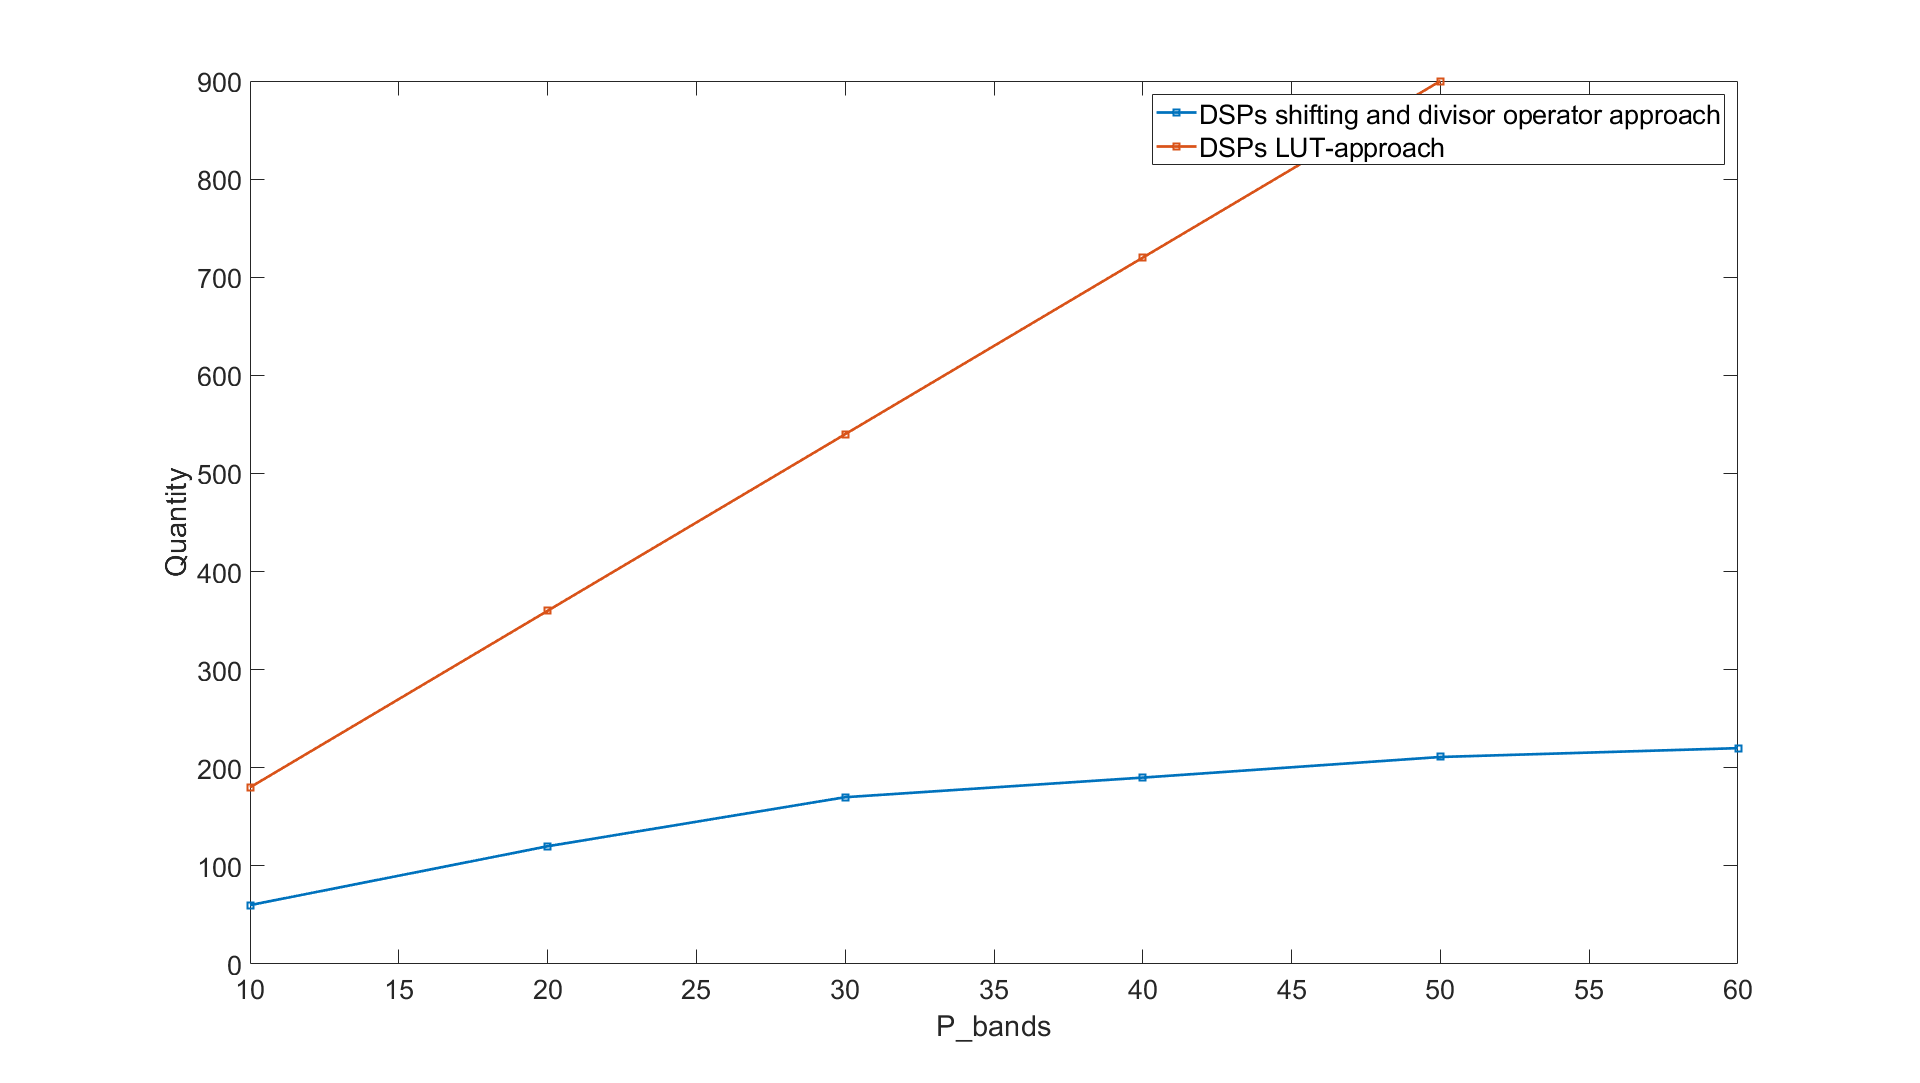
\includegraphics[scale=0.27]{images/syntese_resultat/inverse/number_of_dsps.png}}
  \caption{Number of DSP48E1 synthesized for the \textbf{Inverse} block. } 
  \label{fig:dsps_inverse}
\end{figure}


\begin{figure}[H]

\hbox{\hspace*{-1cm}                                                           
   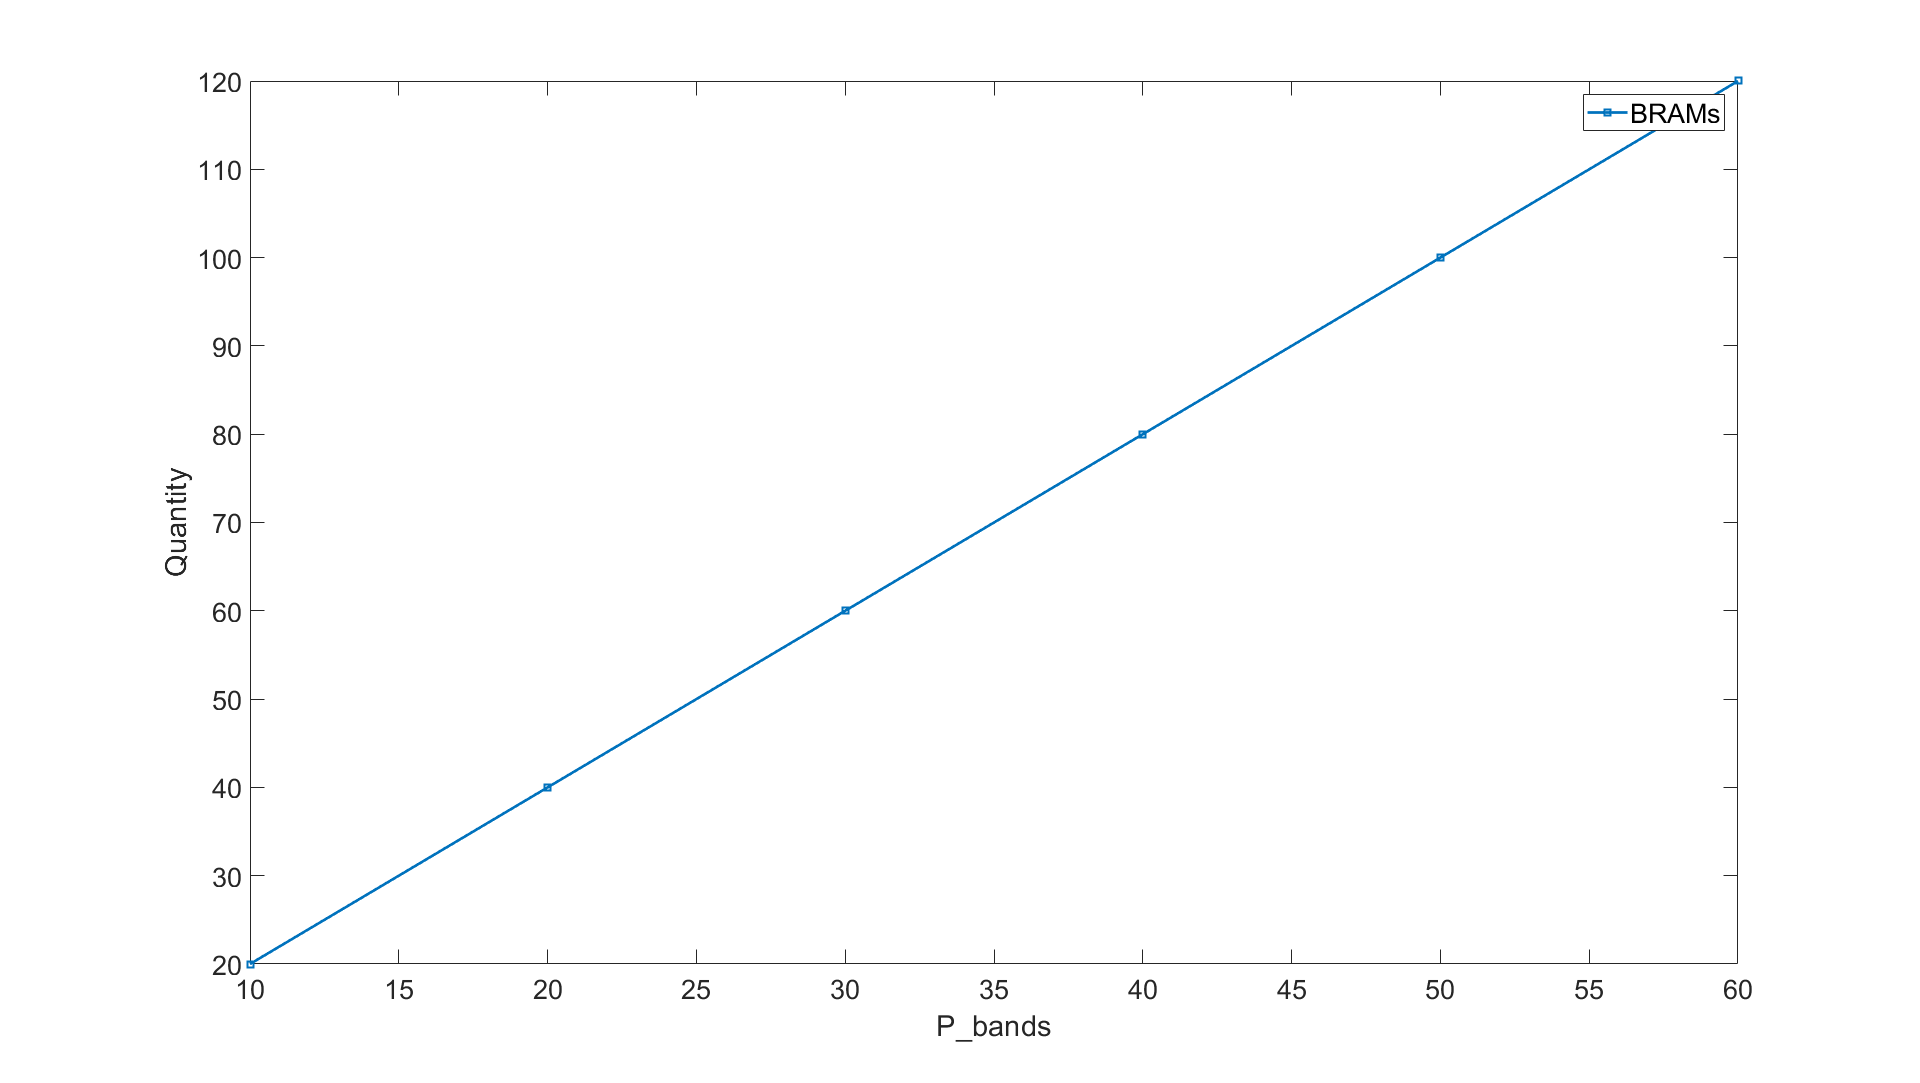
\includegraphics[scale=0.27]{images/syntese_resultat/inverse/brams.png}}
  \caption{Number of BRAMs synthesized for the \textbf{Inverse} block. } 
  \label{fig:brams_inverse}
\end{figure}


\begin{figure}[H]

\hbox{\hspace*{-2cm}                                                           
   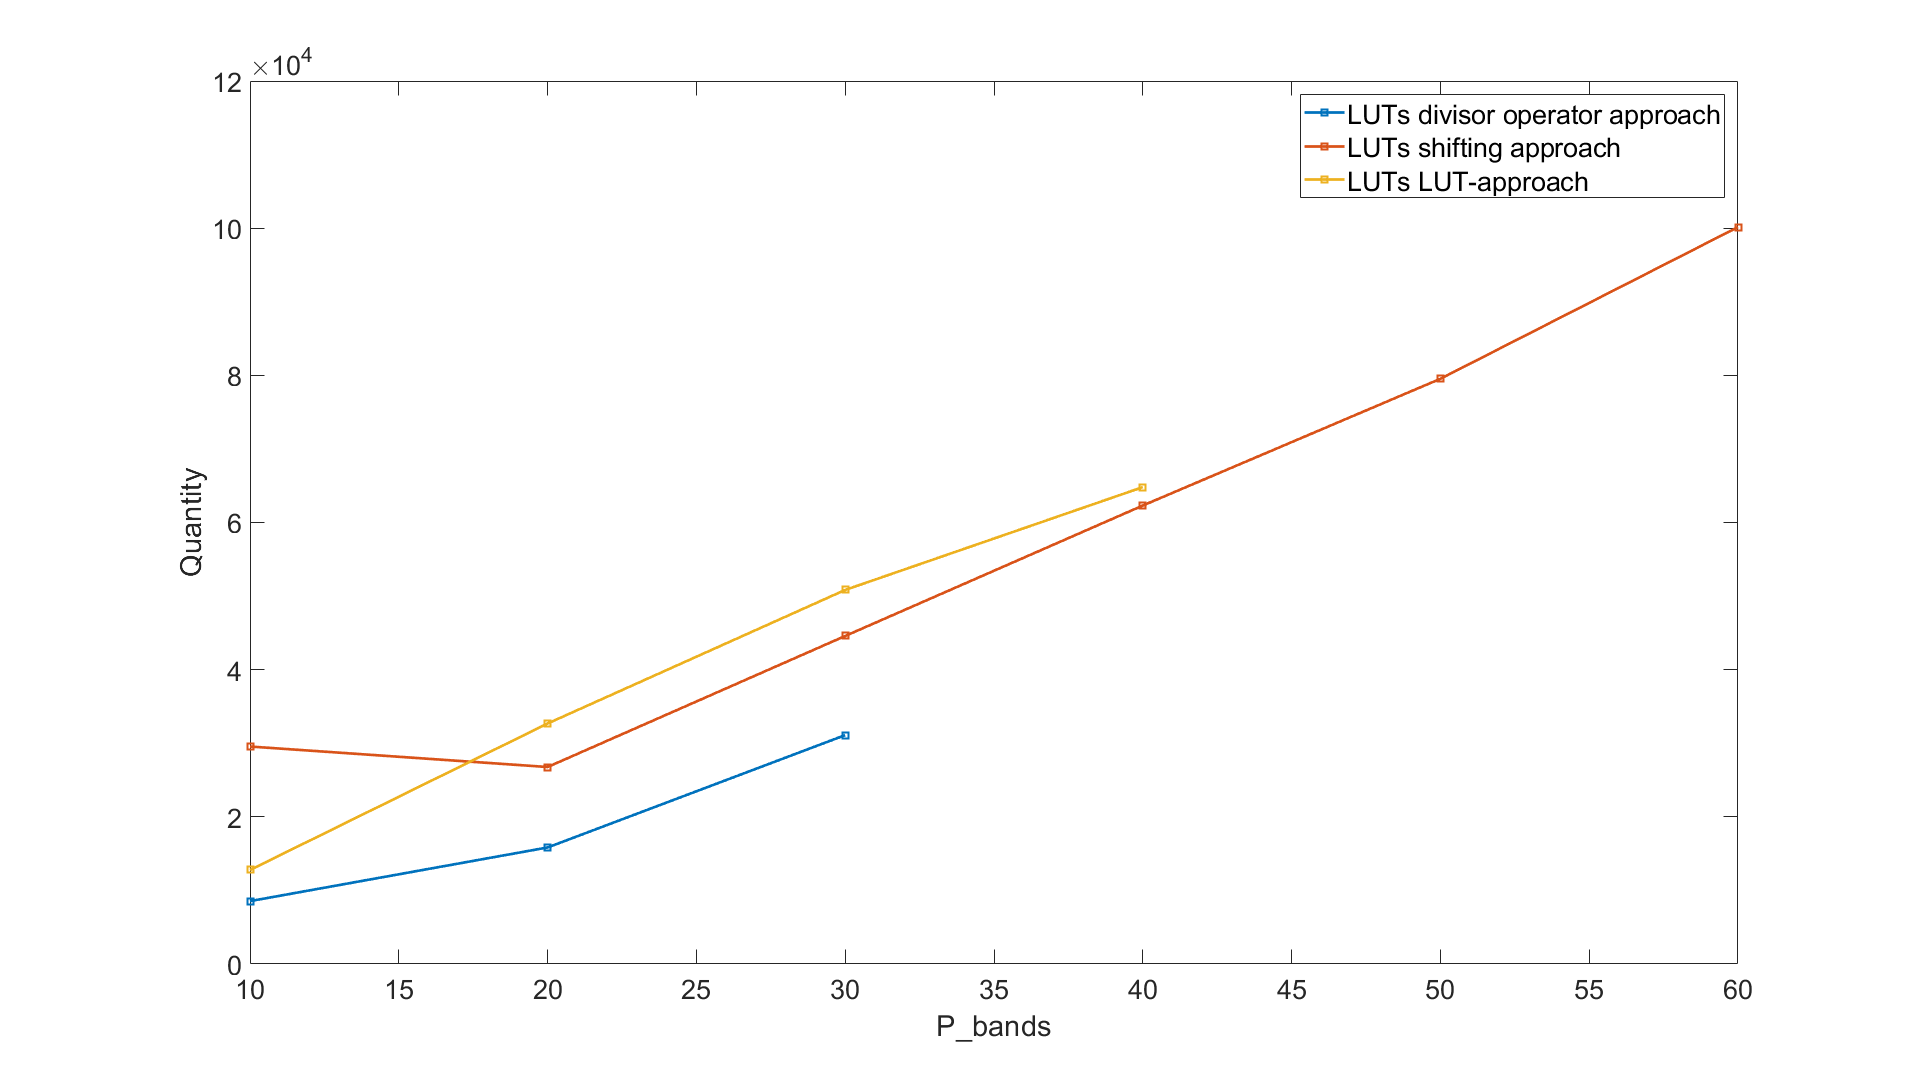
\includegraphics[scale=0.3]{images/syntese_resultat/inverse/number_of_luts.png}}
  \caption{Number of LUTs synthesized for the \textbf{Inverse} block. } 
  \label{fig:luts_inverse}
\end{figure}


\begin{figure}[H]

\hbox{\hspace*{-2cm}                                                           
   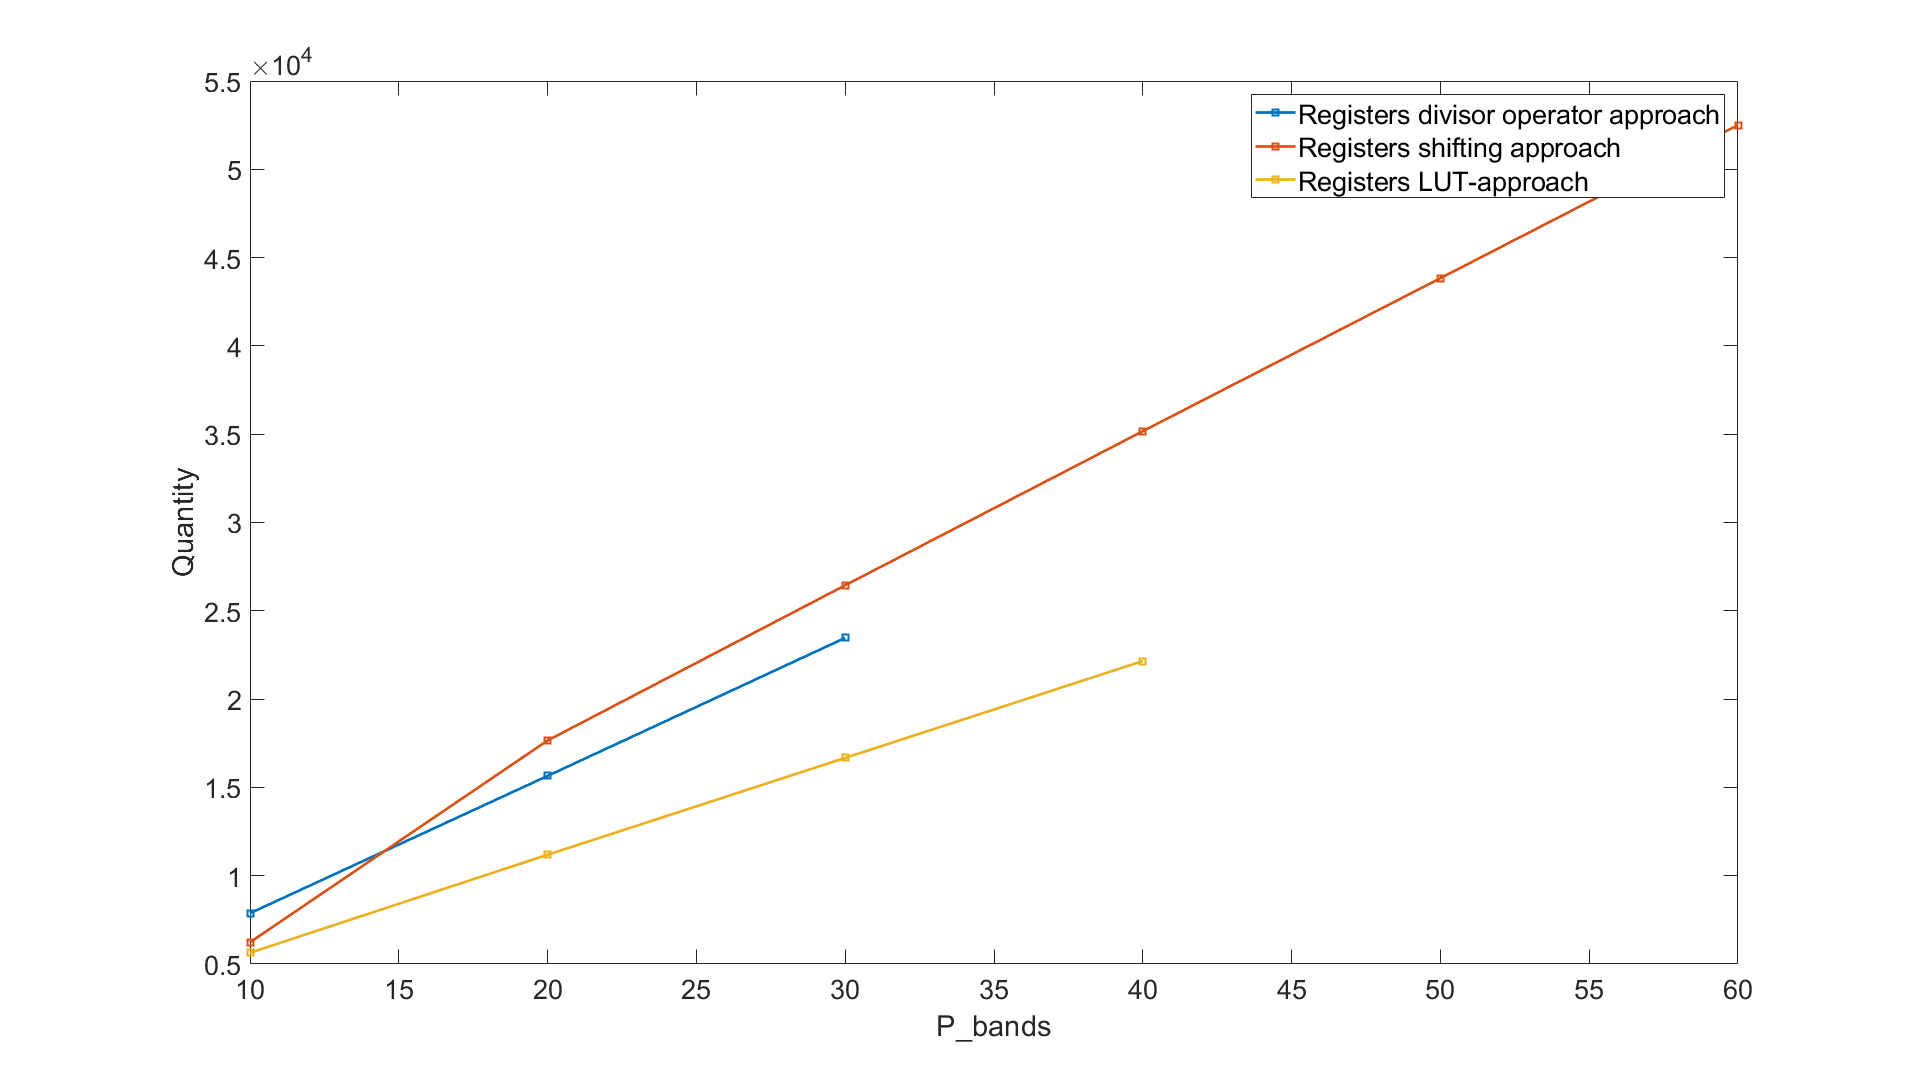
\includegraphics[scale=0.3]{images/syntese_resultat/inverse/number_of_registers.png}}
  \caption{Number of registers synthesized  for the \textbf{Inverse} block.. } 
  \label{fig:registers_inverse}
\end{figure}




%\subsubsection{LUTs and registers}
%\label{sec:synthesis:luts_and_registers_inverse}
%Synthesis results for the first and the second implementation approach of the Gauss-Jordan elimination is shown in Figure \ref{fig:synthesis_result_naive_inverse}.
%
%\begin{figure}[H]
%\hbox{\hspace*{-2cm}                                                           
%
%   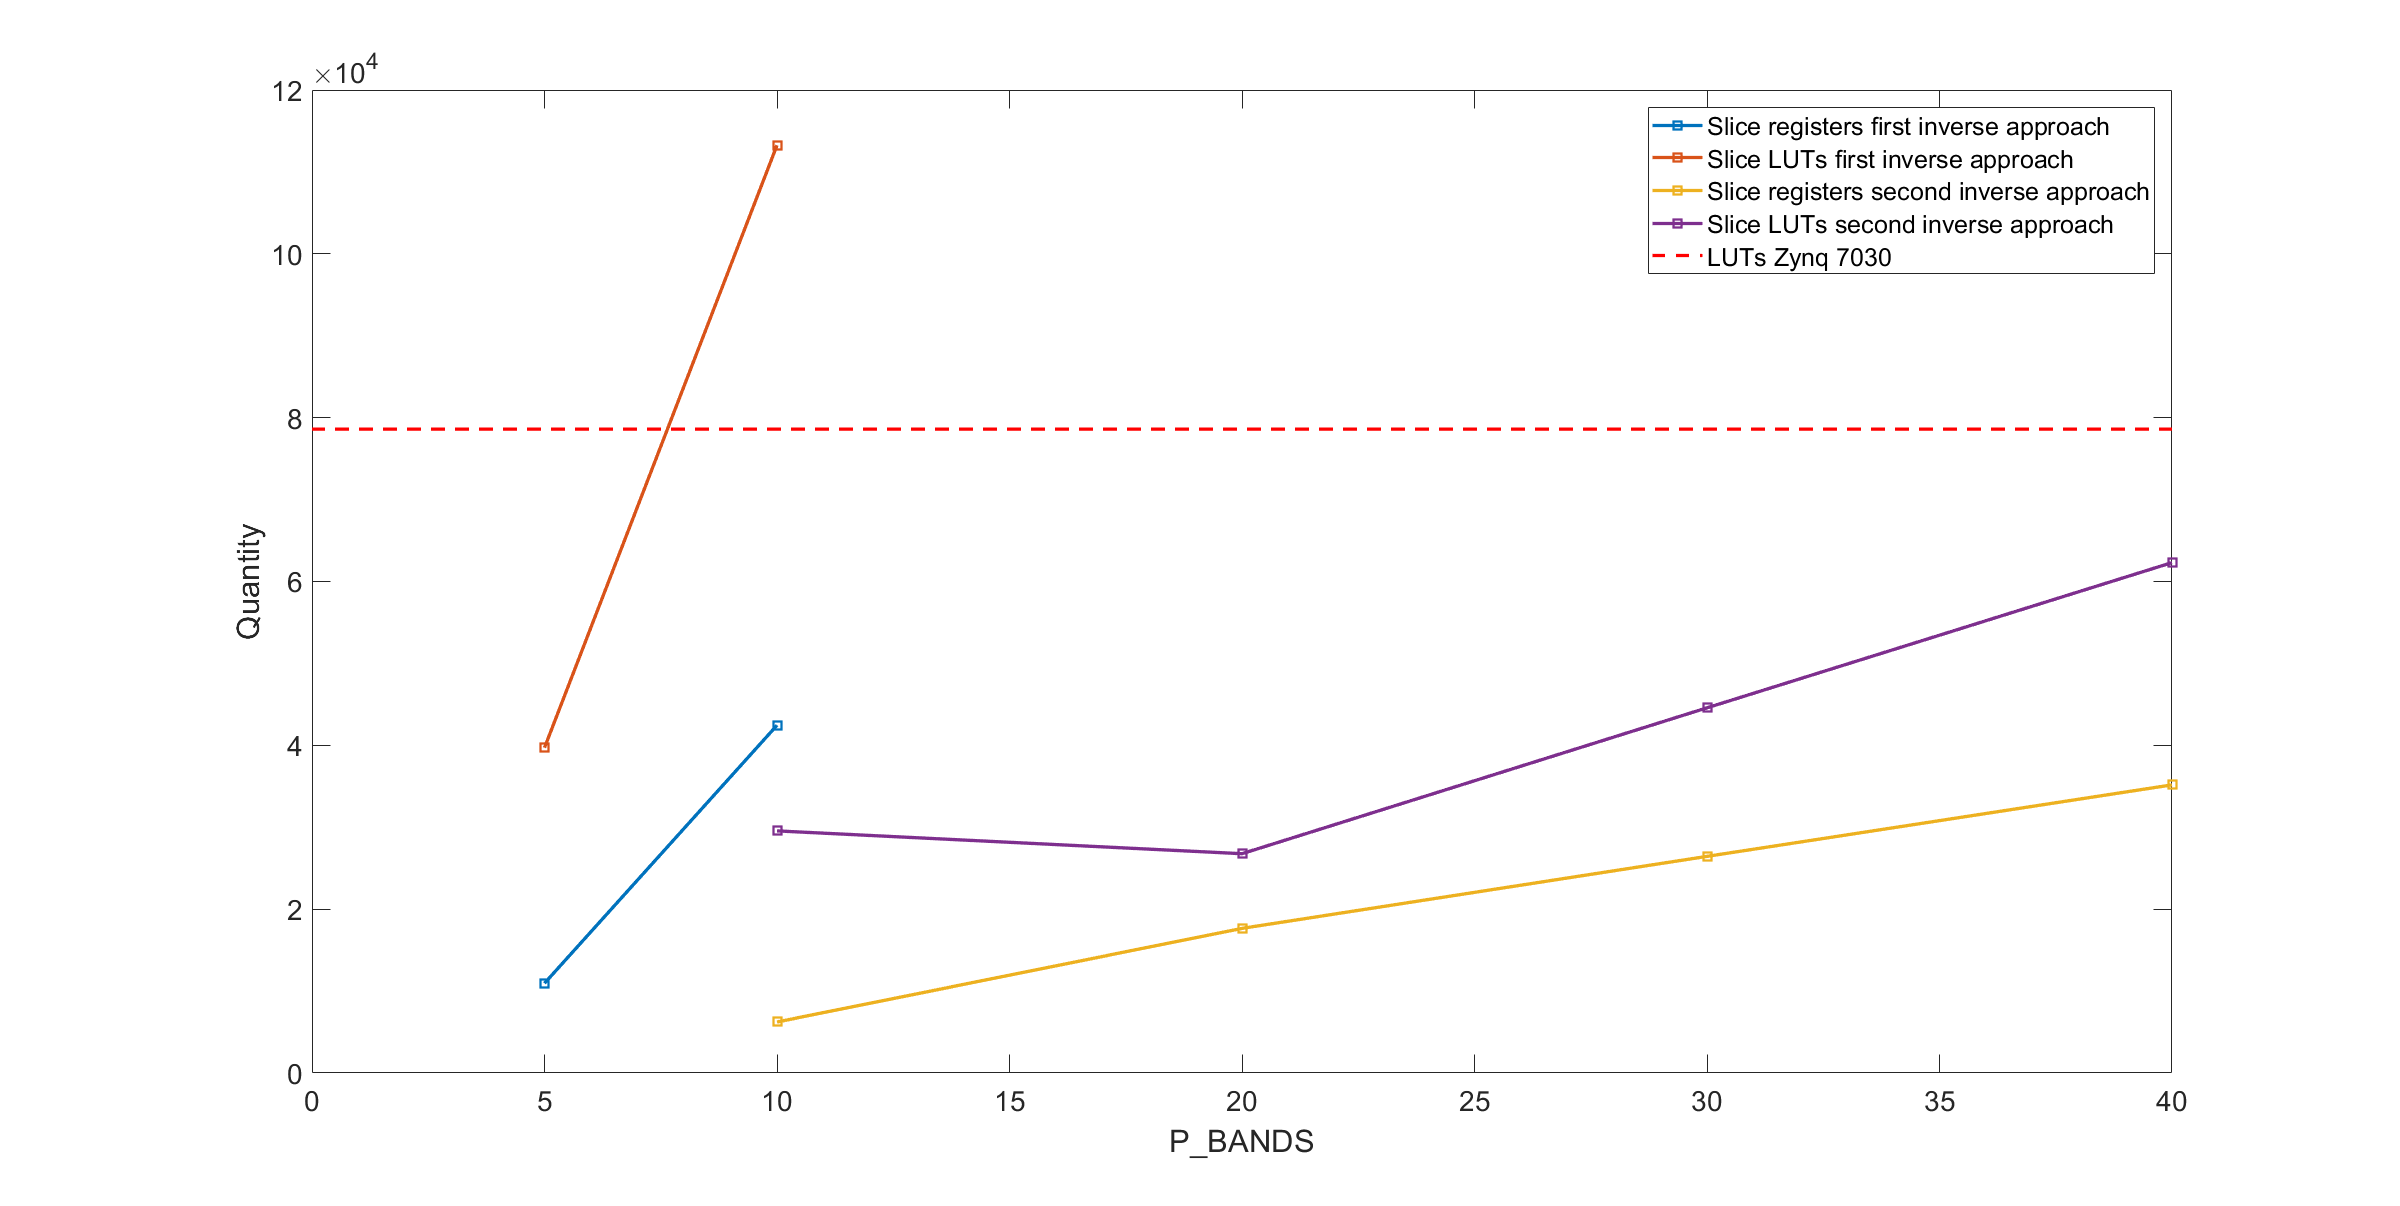
\includegraphics[scale=0.3]{images/inverse_hw/inverse_matrix_luts_and_registers.png}}
%  \caption{Synthesis result for the first and second Gauss-Jordan implementation approach, showing number of LUTs and registers synthesized.  } 
%  \label{fig:synthesis_result_naive_inverse}
%\end{figure}

\subsection{Division timing results}
\subsubsection{Worst Negative Slack division operator}
Implementing division by the use of the division operator "/" yielded the timing results presented in Table \ref{tab:division_operator_wns} when synthesizing block \textbf{Last division}, computing the product $C= B*\frac{1}{A}$. Data width for factor $B$ is 32 bit. The design was synthesized for dividend and divisor data width of 32, 8, 6 and 5, with a target clock constraint of 100 MHz. The target device was the Zedboard Zynq Evaluation and Development kit. 
\begin{table}[H]
    \centering
     \resizebox{1.\textwidth}{!}{
    \begin{tabular}{c|c|c}
    \textbf{Data width divisor and dividend} &\textbf{WNS[ns]}&\textbf{Max frequency[MHz] } \\
         32&-80.524&11.046 \\
         8 & -11.776&45.934 \\
         6&-7.071& 58.578\\
         5 & -5.730&63.572 \\
         
    \end{tabular}}
    \caption{Synthesis results for ZedBoard Zynq Evaluation and Development Kit for \textbf{Last division} using division operator "/".}
    \label{tab:division_operator_wns}
\end{table}
\subsubsection{Worst Negative Slack Adaptive Shifting}
 The design shown in Figure \ref{fig:adaptive_shifting} was synthesized for Zedboard Zynq Evaluation and Development kit Z7020 to check timing for $P\_bands$= [10, 20, 30, 40, 50, 60]. The worst WNS was 2.034 ns, which yields $f_{max}$ of \approx 125 MHz. 
 
 %The max logic delay was $6.932$ns which gives a max operating frequency of 144.25 MHz, not accounting for net delay. 
 
 
 \subsubsection{Worst Negative Slack LUT approach}
 The \textbf{Inverse} block was synthesized for Zedboard Zynq Evaluation and Development kit 7020 with $Div\_Precision$ = 17 and $P\_bands$ =10. The synthesis results yielded a WNS of -5.972 ns. 4.847 of this is net delay. \\
 
$P\_bands$ =10 was chosen due to the LUT-approach over-utilizing DSP48E1 for higher number of $P\_bands$. Over-utilization leads to logic being mapped to LUTs instead of DSP48E1s, leading to wrongful timing results, as described in \cite{cite:dsp_overutilizing}. 
 
 
 \section{Simulation}
% The designs have been tested on simulation runs in Vivado.  
 
 \subsection{ACAD correlation}

 Constrained random input simulation of \textbf{ACAD correlation} has been done in Vivado, and the captured waveforms has been visually inspected. The waveforms shown in Figure \ref{fig:simulation_results_correlation_one} and \ref{fig:simulation_results_correlation_two} shows simulations of input pixel vectors of size $P\_bands$ =4, $Pixel\_data\_width$ =16.\\
 
 Figure \ref{fig:simulation_results_correlation_one} shows a simulation for a data input pixel vector of [0x00ff, 0x00f9, 0x00a5, 0x0055]. This is simulated to be the first pixel of the hyperspectral image.\\
 
 Figure \ref{fig:simulation_results_correlation_one} shows a simulation for a data input pixel vector of [0x0015, 0x00aa, 0x0029, 0x0009]. This is simulated to be the second pixel of the hyperspectral image.
 
 



\begin{figure}[H]
\refstepcounter{figure}
\begin{tabular}{c|c}

   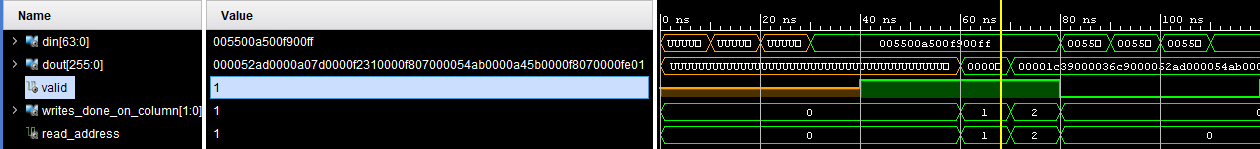
\includegraphics[scale=0.6, angle=90, origin=c]{images/simulation_results/correlation_pixel_one.PNG}
   \rotatebox[origin=c]{90}{ Figure~\thefigure: Simulation of the \textbf{ACAD correlation} block.}
  %\caption{ \textbf{ROTATE}FSM controlling the architecture shown in Figure  } 
  \end{tabular}
  \label{fig:simulation_results_correlation_one}
\end{figure}


\begin{figure}[H]
\refstepcounter{figure}
\begin{tabular}{c|c}

   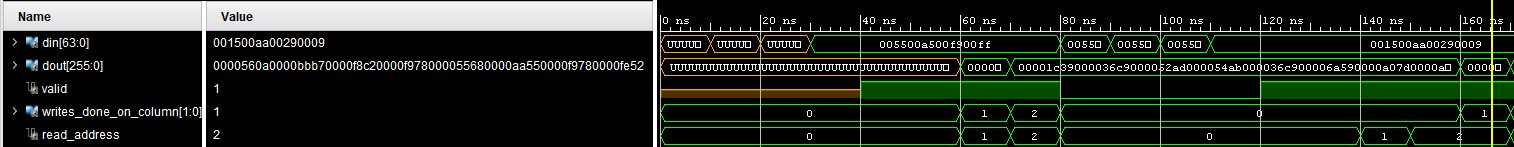
\includegraphics[scale=0.5, angle=90, origin=c]{images/simulation_results/correlation_pixel_two.PNG}
   \rotatebox[origin=c]{90}{ Figure~\thefigure: Simulation of the \textbf{ACAD correlation} block.}
  %\caption{ \textbf{ROTATE}FSM controlling the architecture shown in Figure  } 
  \end{tabular}
  \label{fig:simulation_results_correlation_two}
\end{figure}


 
 \subsection{Inverse}
 Simulation has been done with $P\_bands$=[4,6] and $Pixel\_data\_width$= 16, with constrained random input.  Figure \ref{fig:simulation_results_inverse} shows a simulation with $P\_bands$ = 4.   


\begin{figure}[H]
\refstepcounter{figure}
\begin{tabular}{c|c}

   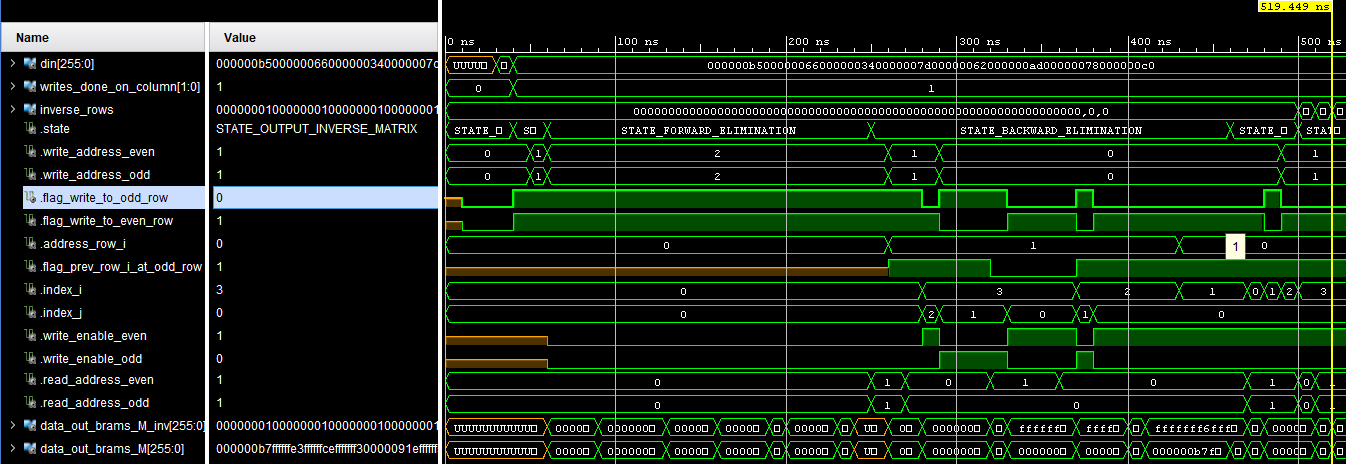
\includegraphics[scale=0.6, angle=90, origin=c]{images/simulation_results/complete_inverse_bram_approach_4_by_4_matrix_formatted_for_latex.png}
   \rotatebox[origin=c]{90}{ Figure~\thefigure: Simulation of the \textbf{Inverse} block.}
  %\caption{ \textbf{ROTATE}FSM controlling the architecture shown in Figure  } 
  \end{tabular}
  \label{fig:simulation_results_inverse}
\end{figure}

